\section{Arhitektura sustava i implementacija}
\label{chap:implementacija}

Nakon definiranja teorijskih osnova i formalizacije problema, ovo poglavlje detaljno opisuje praktičnu realizaciju razvijenog optimizacijskog modela. Ovo poglavlje predstavlja most između teorijske formulacije problema iz Poglavlja 3 i empirijske evaluacije rezultata koja slijedi u Poglavlju 5, detaljno prikazujući kako je apstraktni model preveden u operativni računalni sustav. Sustav je implementiran u programskom jeziku Python (verzija 3.x), odabranom zbog čitljivosti, bogatog ekosustava biblioteka i široke primjene u znanstvenom računarstvu \cite{PythonSoftwareFoundation}. U nastavku se opisuje arhitektura programskog rješenja, korištene tehnologije te detalji implementacije ključnih komponenata.
\subsection{Korištene tehnologije i biblioteke}
Za izradu sustava korišten je niz standardnih biblioteka iz Python ekosustava za znanstveno računarstvo. Biblioteka DEAP \cite{DEAP2012} korištena je kao temeljni okvir za implementaciju genetskog algoritma. Za numeričke operacije i statističku obradu korišten je NumPy \cite{Harris2020}, dok je za manipulaciju i spremanje tabličnih podataka korišten Pandas \cite{PandasDevelopmentTeam2020}. Vizualizacija rezultata provedena je pomoću biblioteka Seaborn \cite{Waskom2021} i Matplotlib \cite{Hunter2007}. Modeliranje nesigurnosti pomoću Trokutaste distribucije implementirano je korištenjem standardne Python biblioteke Random. Detaljan pregled dan je u Tablici \ref{tab:biblioteke}.
\begin{table}[H]
\centering
\caption{Korištene biblioteke u implementaciji}
\label{tab:biblioteke}
\begin{tabular}{|l|p{10cm}|}
\hline
\textbf{Biblioteka} & \textbf{Namjena i citat} \\ \hline
Python & Osnovni programski jezik za cjelokupnu implementaciju. \cite{PythonSoftwareFoundation} \\ \hline
DEAP & Okvir za razvoj i provedbu evolucijskih algoritama. \cite{DEAP2012} \\ \hline
NumPy & Numeričke operacije i statistička obrada nizova podataka. \cite{Harris2020} \\ \hline
Pandas & Učitavanje, obrada i spremanje tabličnih podataka s rezultatima. \cite{PandasDevelopmentTeam2020} \\ \hline
Seaborn & Kreiranje naprednih statističkih vizualizacija (stupčasti, linijski i raspršeni grafikoni). \cite{Waskom2021} \\ \hline
Matplotlib & Osnovna biblioteka za crtanje na koju se oslanja Seaborn. \cite{Hunter2007} \\ \hline
Random & Standardna Python biblioteka korištena za generiranje slučajnih brojeva i uzorkovanje iz Trokutaste distribucije. \\ \hline
\end{tabular}
\end{table}

\subsection{Arhitektura eksperimentalnog okvira}

Sustav razvijen za potrebe ovog rada nije zamišljen kao monolitna skripta, već kao cjeloviti i modularni eksperimentalni okvir. Takva arhitektura, prikazana na Slici \ref{fig:tok_istrazivanja}, omogućuje sustavnu analizu, kalibraciju i usporedbu optimizacijskih metodologija kroz dvo-fazni proces istraživanja. Okvir se sastoji od dva glavna analitička modula koji slijede dvo-fazni pristup istraživanju, te jednog pomoćnog modula za obradu i prikaz rezultata.

Prvi modul, \textbf{Modul za analizu i kalibraciju genetskog algoritma}, predstavlja temelj istraživanja i odgovara na pitanje: \emph{``Kako optimalno konfigurirati genetski algoritam za rješavanje zadanog problema?''}. Njegova primarna svrha je provođenje detaljne ablacijske studije kojom se ispituje utjecaj svakog ključnog parametra na performanse. Kroz višestruka pokretanja različitih konfiguracija (standardni GA, bez križanja, bez mutacije, s povećanim brojem generacija, s većom populacijom), izračunavanjem metrika performansi, uključujući prosječnu vrijednost (mean) i standardnu devijaciju (std) za ROI i procijenjeno trajanje, ovaj modul kao izlaz generira "šampionsku" konfiguraciju – skup optimalnih parametara koji osiguravaju najbolje performanse i koji se koriste u daljnjoj analizi.

    Drugi, ključni modul je \textbf{Modul za usporednu analizu optimizacijskih scenarija}. On čini srž diplomskog rada i koristi "šampionsku" konfiguraciju za provođenje konačne, statistički robusne usporedbe triju različitih pristupa rješavanju problema: osnovnog modela nasumične pretrage, klasičnog genetskog algoritma usmjerenog isključivo na ROI, te hibridnog GA+MC modela (NSGA-II) koji provodi više-kriterijsku optimizaciju koja istovremeno maksimizira ROI i minimizira rizik trajanja procijenjen Monte Carlo simulacijom.  Izlaz ovog modula je konačna tablica s usporednim rezultatima performansii(ROI, trajanje) i stabilnosti(standardna devijacija) za svaki od triju scenarija.

    Treći, \textbf{Modul za obradu i vizualizaciju rezultata}, služi kao pomoćni alat za interpretaciju podataka dobivenih iz prva dva modula. Njegova funkcionalnost obuhvaća obradu i transformaciju sirovih podataka u pregledne tablice pomoću biblioteke \texttt{pandas}, što olakšava strukturiranje rezultata i spremanje u CSV format. Za stvaranje grafičkih prikaza, kao što su stupčasti dijagrami za usporedbu prosječnih vrijednosti, 2D raspršeni dijagrami za prikaz Paretovog fronta ili dijagrami konvergencije, korištene su snažne biblioteke \texttt{matplotlib} i \texttt{seaborn}. Dok \texttt{matplotlib} pruža temelje za stvaranje raznih tipova grafova, \texttt{seaborn}, izgrađen na njemu, nudi naprednije statističke prikaze i atraktivniji, profesionalni izgled uz minimalno kodiranje.

    Osim spomenutih funkcionalnosti, ključan zadatak ovog modula je \textbf{analiza i vizualizacija konvergencije algoritma}. Ova analiza pruža neposredan dokaz da je evolucijski proces bio uspješan. Konvergencija se prati kroz sve generacije bilježenjem promjena u fitnes vrijednostima (ROI-u) najbolje jedinke u svakoj generaciji. Uspješna konvergencija manifestira se u obliku krivulje koja naglo raste u početnim generacijama, a zatim se postupno izravnava, što ukazuje na to da je algoritam pronašao optimalno ili blizu-optimalno rješenje i da daljnja evolucija ne donosi značajna poboljšanja.

Vizualni prikaz konvergencije, koji stavlja fitnes vrijednost na Y-os, a broj generacije na X-os, ključan je alat za potvrdu da algoritam nije stagnirao i da je dosegnuo stabilno stanje. Također pomaže u određivanju optimalnog broja generacija potrebnih za rješavanje problema, čime se direktno utječe na računalnu efikasnost. Na taj način, ovaj modul ne samo da prikazuje konačne rezultate, već i pruža uvid u sam proces optimizacije.   

\begin{figure}[H]
    \centering
    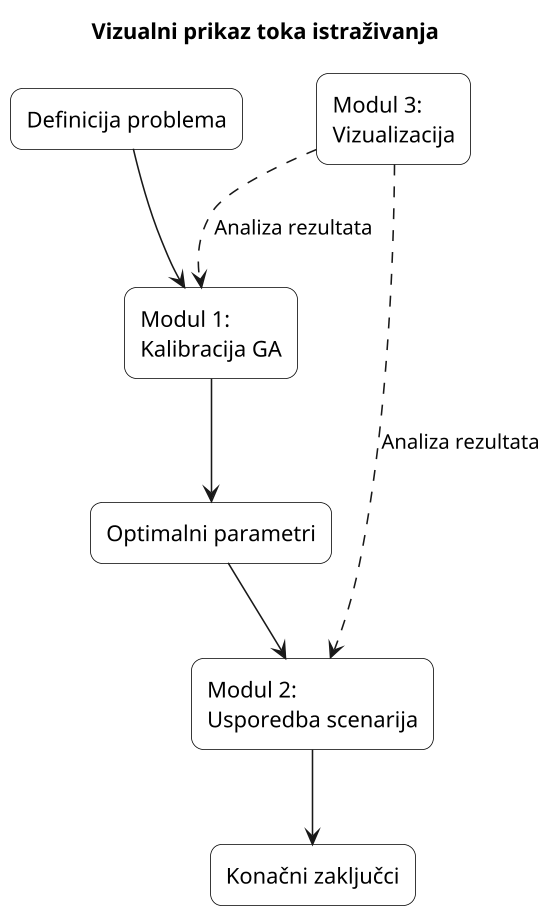
\includegraphics[width=0.9\textwidth]{slike/tijek_istrazivanja.png}
    \caption{Vizualni prikaz toka istraživanja}
    \label{fig:tok_istrazivanja}
\end{figure}
\subsection{Implementacija ključnih komponenti}
\subsubsection{Modeliranje nesigurnosti: Monte Carlo simulacija}

Za svaku projektnu aktivnost definirane su tri točke procjene trajanja:
\[
a \ (\text{optimistična}), \quad
m \ (\text{najvjerojatnija}), \quad
b \ (\text{pesimistična})
\]
Iako u teoriji postoje kompleksnije distribucije poput \textit{Beta-PERT} distribucije, 
za potrebe ovog rada odabrana je \textbf{Trokutasta distribucija (Triangular distribution)} 
zbog svoje praktičnosti, računalne efikasnosti i intuitivnog temelja na tri poznate procjene.
Standardna Python biblioteka \texttt{random} pokazala se dovoljnom za generiranje trokutastih distribucija, eliminirajući potrebu za dodatnim, kompleksnijim bibliotekama, što doprinosi jednostavnosti i prenosivosti koda. Ključno je napomenuti da se stohastička komponenta (simulacija) izvršava unutar determinističkog okvira genetskog algoritma, što znači da se svaka jedinka evaluira na temelju statistički stabilne prosječne vrijednosti trajanja, a ne na temelju jedne slučajne procjene
\paragraph{Generiranje trajanja aktivnosti.}
U svakoj iteraciji Monte Carlo simulacije, trajanje svake aktivnosti generira se slučajnom vrijednošću 
unutar raspona $[a, b]$ s najvećom vjerojatnošću u točki $m$.  
Trokutasta distribucija definirana je funkcijom gustoće vjerojatnosti:
\[
f(x) =
\begin{cases}
\frac{2(x-a)}{(b-a)(m-a)}, & a \leq x < m, \\
\frac{2(b-x)}{(b-a)(b-m)}, & m \leq x \leq b, \\
0, & \text{inače}.
\end{cases}
\]

\paragraph{Procjena trajanja portfelja.}
Ukupno trajanje projektnog portfelja u jednoj simulaciji dobiva se zbrojem trajanja svih aktivnosti odabranih u tom portfelju:
\[
T_{\text{portfolio}} = \sum_{i \in S} t_i
\]
gdje je $S$ skup odabranih aktivnosti, a $t_i$ generirano trajanje aktivnosti $i$.

Implementacija se temelji na \texttt{monte\_carlo\_eval\_duration} funkciji prikazanoj u Isječku koda \ref{lst:monte_carlo}, koja predstavlja konkretnu realizaciju teorijskog procesa opisanog u Poglavlju 2. 

Objašnjenje \textbf{Isječka koda \ref{lst:monte_carlo}}:

Funkcija \texttt{monte\_carlo\_eval\_duration} predstavlja srce Monte Carlo simulacije. Njezina je svrha procijeniti očekivano trajanje zadanog portfelja projekata, uzimajući u obzir inherentnu nesigurnost.

\begin{lstlisting}[float, language=Python, caption={Funkcija za Monte Carlo procjenu trajanja}, label={lst:monte_carlo}, captionpos=b]
def monte_carlo_eval_duration(individual, activities, config):
    selected = [act for i, act in enumerate(activities) if individual[i] == 1]
    if not selected:
        return 0.0
    durations = [
        sum(
            random.triangular(act["optimistic"], act["realistic"], act["pessimistic"])
            for act in selected
        )
        for _ in range(config["NUM_SIMULATIONS"])
    ]
    return np.mean(durations)
\end{lstlisting}

\begin{description}
    \item[\texttt{def monte\_carlo\_eval\_duration(individual, activities, config):}] Definira funkciju koja prihvaća tri ključna ulazna parametra: \texttt{individual} (binarni niz koji predstavlja jedinku, tj. odabrani portfelj), \texttt{activities} (lista svih dostupnih projekata) i \texttt{config} (rječnik s postavkama, npr. broj simulacija).
    \item[\texttt{selected = [act for i, act in enumerate(activities) if individual[i] == 1]}] Ova linija koristi *list comprehension* kako bi, na temelju binarne reprezentacije \texttt{individual} jedinke, stvorila novu listu koja sadrži samo objekte (rječnike) za odabrane projekte.
    \item[\texttt{if not selected: return 0.0}] Jednostavna provjera koja osigurava da funkcija pravilno postupa s praznim portfeljima, vraćajući \texttt{0.0} kao njihovo trajanje.
    \item[\texttt{durations = [...]}] Ovaj dio je srž simulacije. Vanjska *list comprehension* \texttt{for \_ in range(config["NUM\_SIMULATIONS"])} osigurava da se proces ponovi točno onoliko puta koliko je zadano u konfiguraciji. Unutarnja petlja \texttt{for act in selected} prolazi kroz svaki odabrani projekt u jednoj simulaciji.
    \item[\texttt{random.triangular(act["optimistic"], act["realistic"], act["pessimistic"])}] Ovo je ključni poziv funkciji iz Pythonove \texttt{random} biblioteke. Ona generira jednu slučajnu vrijednost trajanja za svaki projekt, koristeći njegove tri točke procjene (optimistična, najvjerojatnija, pesimistična).
    \item[\texttt{sum(...)}] Suma se koristi za zbrajanje trajanja svih projekata u toj jednoj simulaciji, čime se dobiva jedno moguće ukupno trajanje portfelja.
    \item[\texttt{return np.mean(durations)}] Konačno, funkcija vraća prosječnu vrijednost svih \texttt{NUM\_SIMULATIONS} trajanja. Ova prosječna vrijednost služi kao statistički pouzdana procjena očekivanog trajanja portfelja i koristi se u funkciji pogodnosti.
\end{description}

\paragraph{Agregiranje rezultata.}
Funkcija za zadani portfelj provodi velik broj simulacija $(\text{NUM\_SIMULATIONS})$. U svakoj simulaciji, za svaku odabranu aktivnost generira se slučajno trajanje iz Trokutaste distribucije, zbrajaju se trajanja unutar te simulacije, a na kraju se vraća prosječna vrijednost svih simuliranih ukupnih trajanja.
\[
\overline{T}(S) = \frac{1}{\text{NUM\_SIMULATIONS}} \sum_{k=1}^{\text{NUM\_SIMULATIONS}} T_{\text{portfolio}}^{(k)}
\]
gdje $T_{\text{portfolio}}^{(k)}$ označava ukupno trajanje portfelja u $k$-toj simulaciji.


\subsubsection{Optimizacijski pristup: Genetski algoritam}

Implementacija genetskog algoritma provedena je pomoću programske biblioteke \texttt{DEAP} (Distributed Evolutionary Algorithms in Python) \cite{DEAP2012}. 
S obzirom na prirodu problema odabira podskupa aktivnosti, korištena je \textbf{binarna reprezentacija}, gdje svaka jedinka (kromosom) predstavlja jedan portfelj projekata u obliku binarnog niza. Vrijednost '1' na poziciji i označava da je $i$-ta aktivnost odabrana, dok '0' označava da nije.
\paragraph{Reprezentacija jedinke.}
Svaka jedinka (kromosom) u populaciji predstavlja jedno potencijalno rješenje – jedan portfelj projekata. 
Predstavljena je kao binarni niz duljine jednake ukupnom broju aktivnosti $(\text{NUM\_ACTIVITIES})$, gdje gen na poziciji $i$ ima vrijednost:
\[
g_i =
\begin{cases}
1, & \text{ako je $i$-ta aktivnost odabrana}, \\
0, & \text{ako nije odabrana}.
\end{cases}
\]
\paragraph{Konfiguracija genetskih operatora (DEAP Toolbox)}

DEAP koristi koncept "kutije s alatima" (\texttt{Toolbox}) za registraciju svih komponenata potrebnih za evolucijski proces. Za ovaj rad, operatori su odabrani na temelju standardnih praksi za binarne genetske algoritme i specifičnosti problema, kako je prikazano u Isječku koda \ref{lst:toolbox}. U nastavku je dano obrazloženje za odabir svakog ključnog operatora.

\paragraph{Selekcija.}
     Za jedno-kriterijsku optimizaciju odabrana je turnirska selekcija \\ (\texttt{tools.selTournament}). Za razliku od drugih metoda poput selekcije ruleta, koja može dovesti do prerane konvergencije ako jedna "super-jedinka" dominira populacijom, turnirska selekcija pruža bolju kontrolu nad "selekcijskim pritiskom" \cite{Goldberg1989}. Korištenjem manjeg turnira (veličine 3), osigurava se da i prosječno dobre jedinke imaju priliku za reprodukciju, što pomaže u očuvanju genetske raznolikosti. Za više-kriterijsku optimizaciju, primjena operatora \texttt{tools.selNSGA2} je nužna jer on ne provodi jednostavnu selekciju, već implementira cjelokupnu logiku sortiranja po nedominaciji i izračuna gustoće naseljenosti, što je srž NSGA-II algoritma opisanog u Poglavlju 2.

\paragraph{Križanje.}
Kao glavni mehanizam rekombinacije, odabrano je dvo-točkovno križanje (\texttt{tools.cxTwoPoint}). Ova metoda predstavlja dobar kompromis između očuvanja dobrih shema (građevnih blokova) i istraživanja novih kombinacija. U usporedbi s jedno-točkovnim križanjem, manje je podložno pozicijskoj pristranosti, dok je istovremeno manje disruptivno od uniformnog križanja, koje može previše lako razbiti uspješne kombinacije gena. Dvo-točkovno križanje se stoga smatra robusnim i pouzdanim izborom za mnoge binarne probleme \cite{Mitchell1998}.

\paragraph{Mutacija.}
Odabrana je standardna mutacija slučajne promjene bita (\texttt{tools.mutFlipBit}). Njena uloga je ključna za istraživanje (exploration) i sprječavanje stagnacije algoritma. Ovaj operator osigurava da za svaku poziciju u kromosomu uvijek postoji mala, ne-nulta vjerojatnost promjene vrijednosti (iz 0 u 1 ili obrnuto). Time se garantira da algoritam može doseći bilo koju točku u prostoru rješenja i sprječava se situacija u kojoj cijela populacija konvergira prema genu iste vrijednosti, iz koje se samo križanjem ne bi mogla oporaviti.

Vjerojatnosti primjene križanja (\texttt{CX\_PB}) i mutacije (\texttt{MUT\_PB}) definirane su kao vanjski parametri u glavnom konfiguracijskom rječniku, što omogućuje njihovo lako podešavanje i testiranje, kao što je i učinjeno u prvoj fazi eksperimenata.

Koncept Toolbox u DEAP biblioteci omogućuje iznimnu modularnost i fleksibilnost. Umjesto da se operatori pozivaju direktno, oni se registriraju u Toolbox objektu pod aliasima (\texttt{mate},\texttt{mutate},\texttt{select},\texttt{evaluate}). Ova 'registracija' stvara apstrakciju koja omogućava lako zamjenjivanje, testiranje i prebacivanje između različitih operatora bez promjene osnovne strukture evolucijskog petlje, što je bilo presudno za fazu kalibracije algoritma u prvom eksperimentu

Objašnjenje \textbf{Isječka koda \ref{lst:toolbox}}:
Ovaj isječak prikazuje konfiguraciju ``kutije s alatima'' (\texttt{Toolbox}) iz \texttt{DEAP} biblioteke.

\begin{lstlisting}[float, language=Python, caption={Primjer konfiguracije DEAP Toolbox-a za genetske operatore.}, label={lst:toolbox}, captionpos=b]

Inicijalizacija Toolbox objekta
toolbox = base.Toolbox()

Registracija operatora za generiranje jedinki i populacije
toolbox.register("attr_bool", random.randint, 0, 1)
toolbox.register("individual", tools.initRepeat, creator.Individual,
toolbox.attr_bool, config["NUM_ACTIVITIES"])
toolbox.register("population", tools.initRepeat, list, toolbox.individual)

Registracija genetskih operatora
toolbox.register("mate", tools.cxTwoPoint)
toolbox.register("mutate", tools.mutFlipBit, indpb=0.1)
toolbox.register("select", tools.selTournament, tournsize=3)
toolbox.register("evaluate", single_objective_fitness)
\end{lstlisting}

\begin{description}
    \item[\texttt{toolbox = base.Toolbox()}] Inicijalizira prazan \texttt{Toolbox} objekt koji će služiti kao registar za sve komponente algoritma.
    \item[\texttt{toolbox.register("attr\_bool", random.randint, 0, 1)}] Registrira funkciju \texttt{random.randint} pod aliasom ``\texttt{attr\_bool}''. Ova funkcija bit će odgovorna za generiranje pojedinačnih gena (0 ili 1) za kromosom.
    \item[\texttt{toolbox.register("individual", tools.initRepeat, creator.Individual, ...)}] Koristi \texttt{tools.initRepeat} za kreiranje cijele jedinke. Drugim riječima, kreira niz gena pozivajući ``\texttt{attr\_bool}'' onoliko puta koliko je zadano brojem projekata (\texttt{NUM\_ACTIVITIES}).
    \item[\texttt{toolbox.register("population", tools.initRepeat, list, toolbox.individual)}] Slično, registrira funkciju za kreiranje populacije, koja se sastoji od ponovljenog pozivanja funkcije ``\texttt{individual}''.
    \item[\texttt{toolbox.register("mate", tools.cxTwoPoint)}, \texttt{toolbox.register("mutate", tools.mutFlipBit, indpb=0.1)}, \texttt{toolbox.register("select", tools.selTournament, tournsize=3)}] Ove tri linije registriraju ključne genetske operatore. Pod aliasima \texttt{mate}, \texttt{mutate} i \texttt{select} skrivaju se specifične funkcije za križanje, mutaciju i selekciju, što omogućuje njihovu laku zamjenu (npr. promjenu iz turnirske selekcije u \texttt{NSGA-II} selekciju).
    \item[\texttt{toolbox.register("evaluate", single\_objective\_fitness)}] Ovo je ključna linija koja povezuje genetski algoritam s funkcijom pogodnosti. Ona govori algoritmu koju funkciju treba pozvati kako bi izračunao ``dobrotu'' svake jedinke, čime se završava priprema za evolucijsku petlju.
\end{description}

\paragraph{implementacija funkcija pogodnosti (Fitness Function).}
Ključni dio implementacije su funkcije pogodnosti. Ovisno o scenariju, korištene su dvije različite funkcije. Za jedno-kriterijsku optimizaciju (GA samo ROI), implementirana je funkcija koja maksimizira ROI i primjenjuje strogu kaznenu metodu za rješenja koja prekoračuju budžet, osiguravajući da su sva nevaljana rješenja lošija od bilo kojeg valjanog.
Za hibridni scenarij (GA+MC), implementirana je više-kriterijska funkcija pogodnosti koja predstavlja srž ovog rada. Kao što je prikazano u Isječku koda \ref{lst:fitness_function}, ova funkcija unutar jedne evaluacije objedinjuje deterministički izračun (ukupni trošak i ROI) i poziv stohastičke Monte Carlo simulacije za procjenu rizika (očekivano trajanje). Vraća tuple s dvije vrijednosti, omogućujući NSGA-II algoritmu da istovremeno optimizira oba cilja.

Objašnjenje \textbf{Isječka koda \ref{lst:fitness_function}}:
Ova funkcija predstavlja srž više-kriterijske optimizacije. Za razliku od jedno-kriterijskog pristupa, ona ne vraća jednu vrijednost, već tuple koji \texttt{NSGA-II} algoritam koristi za rangiranje jedinki i pronalaženje Paretovog fronta.

\begin{lstlisting}[float, language=Python, caption={Više-kriterijska funkcija pogodnosti}, label={lst:fitness_function}, captionpos=b ]
def multi_objective_fitness(individual, activities, config):
    total_cost, total_roi = calculate_metrics(individual, activities)
    if total_cost > config["BUDGET"]:
        return 0, 99999
    avg_duration = monte_carlo_eval_duration(individual, activities, config)
    return total_roi, avg_duration
\end{lstlisting}

\begin{description}
    \item[\texttt{def multi\_objective\_fitness(individual, activities, config):}] Definira funkciju pogodnosti koja prima jedinku, listu aktivnosti i konfiguracijske parametre.
    \item[\texttt{total\_cost, total\_roi = calculate\_metrics(individual, activities)}] Ova linija poziva pomoćnu funkciju \texttt{calculate\_metrics} (čiji kod nije prikazan, ali je opisana njezina funkcija). Ona izračunava ukupni trošak i \texttt{ROI} odabranog portfelja, koristeći determinističke vrijednosti.
    \item[\texttt{if total\_cost > config["BUDGET"]: return 0, 99999}] Ovo je implementacija stroge kaznene funkcije. Ako portfelj prekoračuje budžet, funkcija odmah vraća loše vrijednosti (niski \texttt{ROI}, iznimno dugo trajanje), osiguravajući da \texttt{NSGA-II} algoritam odbaci takva nevaljana rješenja.
    \item[\texttt{avg\_duration = monte\_carlo\_eval\_duration(individual, activities, config)}] Ovo je točka u kojoj se događa stvarna sinergija. Unutar funkcije pogodnosti, koja se poziva za svaku jedinku u svakoj generaciji, poziva se funkcija za Monte Carlo simulaciju kako bi se dobila statistički stabilna procjena trajanja portfelja.
    \item[\texttt{return total\_roi, avg\_duration}] Konačno, funkcija vraća `tuple` s dvije vrijednosti: izračunatim \texttt{ROI}-em i procijenjenim trajanjem. Ove dvije vrijednosti predstavljaju dva optimizacijska cilja (maksimizacija \texttt{ROI}-a i minimizacija trajanja) na temelju kojih \texttt{NSGA-II} rangira jedinke i pretražuje prostor rješenja.
\end{description}

Ovisno o eksperimentalnom scenariju, korištene su dvije vrste funkcije pogodnosti:
\begin{enumerate}
    \item \textbf{Jedno-kriterijska optimizacija.}  
U scenariju GA (samo ROI), algoritam se suočava s klasičnim problemom ograničene optimizacije (\textit{constrained optimization}). Budući da su genetski algoritmi u svojoj osnovi neograničeni pretraživači prostora rješenja, potreban je mehanizam koji će populaciju "usmjeriti" prema rješenjima koja zadovoljavaju zadane uvjete – u ovom slučaju, ograničenje budžeta. Najčešći pristup za rješavanje ovog problema je korištenje kaznenih funkcija (\textit{penalty functions}), koje smanjuju fitness nevaljanih rješenja \cite{Goldberg1989}.

U ovom radu primijenjena je stroga i direktna kaznena metoda. Ako ukupni trošak odabranog portfelja $S$ ne prelazi budžet, njegova pogodnost jednaka je pozitivnoj vrijednosti ukupnog ROI-a. Međutim, ako je budžet prekoračen, pogodnost postaje negativna vrijednost proporcionalna iznosu prekoračenja:
$$
\text{Fitness}(S) = 
\begin{cases}
    \sum_{i \in S} \text{ROI}_i, & \text{ako } \sum_{i \in S} \text{Trošak}_i \leq \text{Budžet} \\
    -(\sum_{i \in S} \text{Trošak}_i - \text{Budžet}), & \text{ako } \sum_{i \in S} \text{Trošak}_i > \text{Budžet}
\end{cases}
$$
Odabir ovakve "smrtne kazne" (\textit{death penalty}) za nevaljana rješenja, gdje fitness postaje negativan, ima nekoliko prednosti. Prvo, implementacija je jednostavna i računalno efikasna. Drugo, stvara jasnu i oštru granicu između valjanog i nevaljanog prostora rješenja, garantirajući da će evolucijski proces uvijek preferirati bilo koje, pa i najlošije valjano rješenje (s pozitivnim fitnessom) u odnosu na bilo koje nevaljano rješenje (s negativnim fitnessom). Iako u literaturi postoje i napredniji pristupi, poput adaptivnih kazni (gdje se jačina kazne mijenja tijekom evolucije) ili algoritama za popravak (koji pokušavaju "popraviti" nevaljane jedinke), odabrana metoda se pokazala dovoljno robusnom i efikasnom za ovaj tip problema, izbjegavajući uvođenje dodatne složenosti.

Ovakav pristup osigurava da genetski algoritam brzo nauči izbjegavati nevaljana područja i fokusira svoju pretragu na obećavajuće, profitabilne portfelje koji zadovoljavaju ključno poslovno ograničenje.

    \item \textbf{Više-kriterijska optimizacija.}  
Za razliku od jedno-kriterijskog pristupa, hibridni scenarij GA+MC usvaja realističniji, više-kriterijski pogled na problem, prepoznajući da uspjeh projektnog portfelja ne ovisi samo o financijskoj dobiti, već i o vremenskom riziku. Stoga su u ovom naprednom modelu, koji koristi NSGA-II algoritam, definirana dva suprotstavljena optimizacijska cilja:

\begin{enumerate}
    \item Maksimizacija ukupnog povrata na investiciju (ROI), kao mjera profitabilnosti.
    \item Minimizacija prosječnog trajanja portfelja, procijenjenog Monte Carlo simulacijom, kao mjera rizika.
\end{enumerate}

Između ova dva cilja postoji fundamentalan i neizbježan kompromis (\textit{trade-off}). Portfelji koji teže maksimalnom ROI-u često uključuju veći broj aktivnosti ili one koje su dugotrajnije i rizičnije. S druge strane, portfelji koji minimiziraju trajanje obično su manji i konzervativniji, te posljedično imaju nižu ukupnu vrijednost. Zbog ovog konflikta, ne postoji jedno, savršeno rješenje koje je istovremeno najbolje po oba kriterija.
Formalno, ovaj se više-kriterijski optimizacijski problem može zapisati kao:
$$
\begin{cases} 
\max f_1(\mathbf{x}) = \sum_{i \in S(\mathbf{x})} v_i \\ 
\min f_2(\mathbf{x}) = E[T(\mathbf{x})]
\end{cases}
$$
gdje $S(\mathbf{x})$ označava skup odabranih aktivnosti za dani vektor odluke $\mathbf{x}$, a $E[T(\mathbf{x})]$ je očekivano trajanje tog portfelja dobiveno Monte Carlo simulacijom.
U praktičnoj implementaciji, ovo se postiže pomoću funkcije pogodnosti (\texttt{multi\_objective\_fitness}) koja za svaku jedinku ne vraća jednu skalarnu vrijednost, već dvoelementni \textit{tuple} koji sadrži vrijednosti oba cilja (ROI, trajanje). Na temelju tih vektorskih vrijednosti, NSGA-II algoritam, detaljno opisan u Poglavlju 2, rangira populaciju i pretražuje prostor rješenja s ciljem pronalaženja Paretovog fronta – skupa optimalnih kompromisnih rješenja.
\end{enumerate}
\subsection{Vizualizacija i obrada rezultata}

Za analizu i prikaz rezultata dobivenih optimizacijom korištene su biblioteke \texttt{pandas} za tabličnu obradu podataka te \texttt{Seaborn} i \texttt{Matplotlib} \cite{Waskom2021, Hunter2007} za grafičku vizualizaciju. Kombinacija ovih alata odabrana je zbog njihove sinergije i efikasnosti u radu s podacima.
\textbf{Pandas} je korišten kao temelj za organizaciju i manipulaciju eksperimentalnih podataka, omogućujući efikasnu filtraciju, sortiranje i agregiranje sirovih rezultata u strukturirane, pregledne tablice. Njegova snaga leži u mogućnosti brzog izračunavanja ključnih statistika (poput prosjeka i standardnih devijacija) potrebnih za usporedbu modela. Pandas je bio nezamjenjiv u ovoj fazi. Na primjer, nakon svake serije pokretanja algoritma, rezultati su se automatski spremali u \texttt{DataFrame} objekte, što je omogućilo lagano izračunavanje prosječnih vrijednosti i standardnih devijacija za usporedbu performansi. Uz to, Pandas je korišten za čitanje ulaznih podataka iz CSV datoteka, osiguravajući robustan i standardiziran ulazno-izlazni proces.

Za vizualizaciju, \textbf{Matplotlib} je služio kao osnovni "motor" za crtanje, dok je Seabornu dana prednost zbog njegove visoke razine apstrakcije i fokusiranosti na izradu statističkih grafova. Seaborn, izgrađen na Matplotlibu, omogućuje stvaranje estetski privlačnih i informativnih dijagrama s minimalno koda, automatski se brinući o bojama, temama i složenim prikazima odnosa među podacima. Upravo je ta jednostavnost i elegancija bila ključna za učinkovit prikaz rezultata više-kriterijske optimizacije.

Ovaj pristup omogućio je sustavnu prezentaciju statistički obrađenih podataka kroz detaljne tablice te vizualnu usporedbu modela pomoću stupčastih i raspršenih dijagrama. Posebno je značajan prikaz Paretovog fronta, koji jasno ilustrira kompromis (\textit{trade-off}) između maksimizacije ROI-a i minimizacije trajanja, pružajući intuitivan uvid u kvalitetu rješenja dobivenih više-kriterijskom optimizacijom.

Ključni vizualni elementi korišteni u ovom radu uključuju:
\begin{itemize}
    \item \textbf{Tablične prikaze:} Detaljne tablice s konačnim, statistički obrađenim rezultatima usporedbe različitih optimizacijskih scenarija, uključujući osnovne metrike poput prosječnog ROI-a, prosječnog trajanja te raspona vrijednosti.
    \item \textbf{Stupčaste dijagrame:} Koristili su se za vizualnu usporedbu prosječnih vrijednosti (\textit{ROI} i trajanje) između različitih metodologija optimizacije, omogućujući brzu identifikaciju učinkovitijih pristupa.

   \item \textbf{Dijagrame konvergencije:} Linijski dijagrami koji prikazuju evoluciju fitnes vrijednosti najbolje jedinke (ROI-a) kroz generacije. Ovi dijagrami ključni su za potvrdu da algoritam nije stagnirao i da je uspješno konvergirao prema optimalnom rješenju.
    \item \textbf{Raspršene dijagrame (\textit{Scatter Plot}):} Prikaz Paretovog fronta dobivenog NSGA-II algoritmom, koji jasno ilustrira kompromis (\textit{trade-off}) između dvaju suprotstavljenih ciljeva: maksimizacije ROI-a i minimizacije trajanja. Time se omogućuje intuitivna procjena učinkovitosti rješenja.
\end{itemize}

Vizualizacija rezultata odigrala je ključnu ulogu u interpretaciji dobivenih podataka, posebno u scenarijima s više ciljeva, gdje tablični prikazi sami po sebi nisu dovoljni za uočavanje odnosa i kompromisa među varijablama.

Sveobuhvatni metodološki okvir i detaljna implementacija opisana u ovom poglavlju služe kao temelj za daljnju analizu. Precizna konfiguracija sustava, od odabira biblioteka do implementacije prilagođenih genetskih operatora i funkcija pogodnosti, ključna je za osiguravanje pouzdanosti i valjanosti dobivenih rezultata. Ovaj okvir nije samo teorijski model, već robustan eksperimentalni sustav koji omogućuje testiranje i usporedbu različitih optimizacijskih scenarija u kontroliranom okruženju. S uspostavljenom arhitekturom i implementacijom svih ključnih modula, rad je spreman za sljedeću fazu – empirijsku evaluaciju i diskusiju rezultata, što je i fokus sljedećeg poglavlja.
